\documentclass[preprint,12pt]{elsarticle}

%% Use the option review to obtain double line spacing
%% \documentclass[preprint,review,12pt]{elsarticle}

%% Use the options 1p,twocolumn; 3p; 3p,twocolumn; 5p; or 5p,twocolumn
%% for a journal layout:
%% \documentclass[final,1p,times]{elsarticle}
%% \documentclass[final,1p,times,twocolumn]{elsarticle}
%% \documentclass[final,3p,times]{elsarticle}
%% \documentclass[final,3p,times,twocolumn]{elsarticle}
%% \documentclass[final,5p,times]{elsarticle}
%% \documentclass[final,5p,times,twocolumn]{elsarticle}

%% if you use PostScript figures in your article
%% use the graphics package for simple commands
%% \usepackage{graphics}
%% or use the graphicx package for more complicated commands
\usepackage{graphicx}
%% or use the epsfig package if you prefer to use the old commands
%% \usepackage{epsfig}

%% The amssymb package provides various useful mathematical symbols
\usepackage{amssymb}
\usepackage{xcolor}
%% The amsthm package provides extended theorem environments
%% \usepackage{amsthm}

%% The lineno packages adds line numbers. Start line numbering with
%% \begin{linenumbers}, end it with \end{linenumbers}. Or switch it on
%% for the whole article with \linenumbers after \end{frontmatter}.
%% \usepackage{lineno}

%% natbib.sty is loaded by default. However, natbib options can be
%% provided with \biboptions{...} command. Following options are
%% valid:

%%   round  -  round parentheses are used (default)
%%   square -  square brackets are used   [option]
%%   curly  -  curly braces are used      {option}
%%   angle  -  angle brackets are used    <option>
%%   semicolon  -  multiple citations separated by semi-colon
%%   colon  - same as semicolon, an earlier confusion
%%   comma  -  separated by comma
%%   numbers-  selects numerical citations
%%   super  -  numerical citations as superscripts
%%   sort   -  sorts multiple citations according to order in ref. list
%%   sort&compress   -  like sort, but also compresses numerical citations
%%   compress - compresses without sorting
%%
%% \biboptions{comma,round}

% \biboptions{}

%% This list environment is used for the references in the
%% Program Summary
%%
\newcounter{bla}
\newenvironment{refnummer}{%
\list{[\arabic{bla}]}%
{\usecounter{bla}%
 \setlength{\itemindent}{0pt}%
 \setlength{\topsep}{0pt}%
 \setlength{\itemsep}{0pt}%
 \setlength{\labelsep}{2pt}%
 \setlength{\listparindent}{0pt}%
 \settowidth{\labelwidth}{[9]}%
 \setlength{\leftmargin}{\labelwidth}%
 \addtolength{\leftmargin}{\labelsep}%
 \setlength{\rightmargin}{0pt}}}
 {\endlist}

\journal{Computer Physics Communications}

\begin{document}

\newcommand{\onlinecite}[1]{\hspace{-1 ex} \nocite{#1}\citenum{#1}} 
\begin{frontmatter}
%% Title, authors and addresses

%% use the tnoteref command within \title for footnotes;
%% use the tnotetext command for the associated footnote;
%% use the fnref command within \author or \address for footnotes;
%% use the fntext command for the associated footnote;
%% use the corref command within \author for corresponding author footnotes;
%% use the cortext command for the associated footnote;
%% use the ead command for the email address,
%% and the form \ead[url] for the home page:
%%
%% \title{Title\tnoteref{label1}}
%% \tnotetext[label1]{}
%% \author{Name\corref{cor1}\fnref{label2}}
%% \ead{email address}
%% \ead[url]{home page}
%% \fntext[label2]{}
%% \cortext[cor1]{}
%% \address{Address\fnref{label3}}
%% \fntext[label3]{}

\title{Supplementary material for VISROC 2.0: Updated Software for the Visualization of the significance of Receiver Operating Characteristics based on confidence ellipses}

\end{frontmatter}
%% main text
\section{The Receiver Operating Characteristics method}
\label{Intro}
The Receiver Operating Characteristics (ROC) curve is a technique used\cite{hosmer2000, GAR09A,NEWEPL,SPRINGER,CAR11,NAT11B,SARCHRIS12B,nhess12,sarlis2015,feng2022,sarlis2020,raffinetti2021} to estimate the predictability of various complex systems. Briefly, the concept behind the method is as follows\cite{FAW06}:

In the case of binary predictions, there are two classes of events: Positive {\bf p} or Negative {\bf n}, where an event is considered as {\bf p} if its magnitude exceeds a
given threshold $M_t$, otherwise it is classified as {\bf n}. Before the occurrence
of each event, a predictor $\epsilon$ is assigned and a class {\bf P} or {\bf N} for the impending event is decided based on whether $\epsilon$ is larger or smaller than,
respectively, the predictor threshold value $\epsilon_t$. If this hypothesized
class is {\bf P} and the event is {\bf p} we have a successful prediction called
True Positive (TP). If the hypothesized class is {\bf N} and the event is {\bf n} we also have a successful prediction, this time called True Negative (TN). However, if the class is {\bf P} and the event is {\bf n} we have a False Positive (FP) unsuccessful prediction, while if the class is {\bf N} and the event is {\bf p} we have a False Negative (FN) unsuccessful prediction. 


Assuming that we examine $P$ events belonging to the {\bf p} class and $Q$ events belonging to the {\bf n} class, one defines\cite{FAW06} the hit rate (H) as: 
\begin{equation}\label{eq:1}
H\equiv\frac{|TP|}{P}=\frac{|TP|}{|TP|+|FN|},
\end{equation}
and the false alarm rate (F) as:
\begin{equation}\label{eq:2}
F\equiv\frac{|FP|}{Q}=\frac{|FP|}{|FP|+|TN|}.
\end{equation}

The ROC curve is then obtained by plotting $H$ as a function of $F$ while we vary the predictor threshold value, $\epsilon_t$ (see, for example, Fig. 1 of Ref. \cite{visroc1}). The statistical significance of a ROC curve will depend on its deviation from the diagonal where $H=F$ which corresponds on 
average to totally random predictions.

When $P$ and $Q$ are sufficiently large\cite{FEL71b}, we are led, for random predictions, to a
two dimensional Gaussian distribution for $H$ and $F$\cite{visroc1}:
\begin{equation}\label{eq:3}
f(F,H)=\frac{\sqrt{PQ}}{2\pi\epsilon_t
(1-\epsilon_t)}\exp\left[-\frac{Q(F-\epsilon_t)^2+P(H-\epsilon_t)^2}{2\epsilon_t
(1-\epsilon_t)}\right].
\end{equation} 

The confidence regions in this case\cite{BER12} are the confidence ellipses\cite{visroc1}:
\begin{equation}\label{eq:4}
{Q(F-\epsilon_t)^2+P(H-\epsilon_t)^2}=k{\epsilon_t (1-\epsilon_t)},
\end{equation} 
with center $(F,H)=(\epsilon_t,\epsilon_t)$ on the diagonal of
the ROC space. $k$ is a positive parameter signifying the confidence level
with $p_0=\exp(-k/2)$. Varying $\epsilon_t$ within the region $[0,1]$,
the center of the ellipse moves along the diagonal. Thus, we can obtain different
ellipses for a given $p_0$-value. The envelope of these ellipses can be
determined by maximizing $H$ under the condition (\ref{eq:4}) for given values of $F$ and $k$. It turns out that this envelope is also an ellipse. The family of these envelope ellipses is called\cite{visroc1} $k$-ellipses family and it covers the whole ROC space. The $k$-value corresponding to an arbitrary ROC point $(F,H)$ is given by\cite{visroc1}:
\begin{eqnarray}\label{eq:5}
k(F,H)&=&2P(H^2-H)+2Q(F^2-F) \nonumber \\
&+&2\sqrt{[P(H^2-H)+Q(F^2-F)]^2+PQ(F-H)^2}.
\end{eqnarray}

Mason and Graham\cite{MAS02} have shown that the Area Under the Curve (AUC), labelled as $A$, in the ROC plane can be calculated as:

\begin{equation}\label{eq:6}
A=1-\frac{U}{PQ},
\end{equation}
where $U$ follows the Mann-Whitney U-statistics\cite{MAN47}. This means that $U$  equals the sum of the number of cases a number $u_k, k=1, 2, \dots, P$ 
is larger than a number $u'_l, l=1, 2, \dots, Q$ when both $\{u_k\}$ and $\{u_l\}$ originate from the same continuous distribution. For large values of $P$ and $Q$, i.e., when $P$ or $Q$ are greater or equal to 30 and $P+Q\geq 40$, the U-statistics can be approximated\cite{MAS02} by a Gaussian distribution.

By calculating the AUC corresponding to a specific $k$-ellipse, we can estimate its significance level $p$. It has been shown\cite{visroc1} that the AUC can be calculated using the following equation: 
\begin{eqnarray}\label{eq:7}
A(k)= \left(1-\frac{x_1}{2}\right)   +  
\left(\frac{Q}{Q+k}\right)\frac{x_1}{2}\left(x_1-1\right) 
\phantom{aaaaaaaaa}\nonumber \\
+ \frac{1}{2}\left(\frac{1}{Q+k}\right)\sqrt{\frac{k\left(Q+k+P\right)}{P}}
\left\{   \sqrt{Q}  \left[
\left(x_1-\frac{1}{2}\right)\sqrt{\frac{Q+k}{4Q}  - 
\left(x_1-\frac{1}{2}\right)^2} \right. \right. \nonumber \\ \left. \left. 
+\left(\frac{Q+k}{4Q}\right)   \arcsin   \left(2\left(x_1-\frac{1}{2}
\right)\sqrt{\frac{Q}{Q+k}}\right)\right] \right. \phantom{aaaaaaaaaaaaaa}
\nonumber  \\ \left. 
+\frac{1}{4\sqrt{Q}}\left[  \sqrt{kQ} 
+(Q+k)\arcsin \left( \sqrt{\frac{Q}{Q+k}}\right)\right] \right\}
\phantom{aaaaaaaaaaaai}
\end{eqnarray}
where\begin{equation}\label{eq:8}
x_1=\frac{1}{2}+\frac{PQ-k\sqrt{Q(k+Q+P)}}{2Q(k+P)}
\end{equation}

The previous version\cite{visroc1} published in 2014 provided a $FORTRAN$ code called VISROC in order to estimate the statistical significance $p$ in the ROC plane using either Mann-Whitney U-statistics or its Gaussian approximation, if applicable. To do so, for each point $(F,H)$, the authors estimated the $k$ value (Eq. \ref{eq:5}) of the $k$-ellipse that passes through this point. Then, they calculated the AUC $A(k)$ using Eq.(\ref{eq:7}), as well as three $k$-ellipses with $p$-values equal to 10\%, 5\% and 1\%, using Eq. (11) of Ref. [\onlinecite{visroc1}]. The statistical significance $p$ of a user defined area under the ROC curve could also be estimated by the code.

In this paper, we present the updated code for the visualization of the confidence
intervals in the ROC plane. The new code has two versions, in $R$ and in $Python$, and implements a GUI that was not available before. We will discuss each version's characteristics as well as the steps taken to overcome the $FORTRAN$ version's limitations in the subsequent Section.

\section{VISROC Updated Version}

The most important new feature in VISROC 2.0 is the addition of a GUI, rendering the software more user-friendly by allowing the user to perform ROC analysis without the knowledge of a specific programming language. Additionally,  a 
user defined ROC can be inserted through a file containing $(F,H)$ points, a feature that was not available before.

Furthermore, the original $FORTRAN$ code VISROC had an unusual feature during the Gaussian approximation in the extreme case that either $P$ or $Q$ was unity (and the other was greater than $38$). In such cases, the final column of the output file outCL.dat (see Subsection \ref{R}) appeared as NaN, reflecting the fact that the $k$-ellipse with $p$-value $p=1\%$ could not be drawn since all the points of the ROC unit square  corresponded to $k$-ellipses with larger $p$-values.
 To surpass this, we introduce in VISROC 2.0 an upper limit for the AUC of $p=1\%$, where if the calculated AUC is larger than unity, then it will default to the number $1-10^{-15}=0.999999999999999$. Obviously when this upper limit is invoked the resulting $k$-ellipse is very close to the upper horizontal axis of the ROC diagram and hence indiscernible, causing no confusion.  

The code for VISROC 2.0 was written in two programming languages: $R$ and $Python$. In Subsections \ref{R} and \ref{Python}, we will describe how each version works in more detail.

\subsection{$R$ Version}\label{R}

The $R$ version of VISROC 2.0 can either be run locally using the $R$ language environment installed in the user's computer, or be launched as an online application, opening in a browser.

The software tests for package dependencies that need to be installed before running the application and installs them automatically in the required version.

%a) ggplot package: used for data visualization and creating graphics\\
%b) scales package: used to customize axis' appearance and the labels of the legends\\
%c) shiny package: used to build the interactive online application.

The GUI is shown in Fig. \ref{fig:1}. One can see that the user can input the number of positive events $P$, the number of negative events $Q$, and the number $N$ of segments in which the interval $[0,1]$ is divided on a square lattice in the ROC diagram by using the \textit{resolution} field. Furthermore, the value of a user defined AUC for which they would like to find the $p$-value can also be defined, as well as the values $F_1$ and $H_1$ ($H_1 > F_1$) of a user defined point $(F_1,H_1)$ on the ROC diagram, for which the user would like to find the $p$-value of the $k$-ellipse passing through it. In addition, by using the button ``Browse'', the user can insert a file containing $(F,H)$ points.

The main window in Fig. \ref{fig:1} showcases a general graph interpretation, with an added button that helps the user refer back to it after running an example. Finally, a ``Help'' button offers instructions regarding the program's input parameters, as well as the output files and results, the different menus, and the potential error outputs.

In Figure \ref{fig:2}, we showcase an example by inserting a file called example.csv containing some test data. The input files we use are $P=15$, $Q=35$, $N=100$, User Defined AUC$=0.51$, and $(F_1,H_1)=(0.65,0.75)$. The resulted $p$-value for the User Defined AUC is approximately $0.46$.  For the $(0.65,0.75)$ point the $p$-value is approximately $0.17$ with an AUC approximately $0.58$. Finally, for the example.csv input file the $p$-value is approximately $0.01$ with AUC=$0.70$. The ``No fault'' indication signifies that we had correct execution, with reasonable input parameters.

In addition, a Plot(F1, H1) button shows the plot for the $(F_1,H_1)=(0.65,0.75)$ point and the corresponding $k$-ellipse. Finally, the program allows to change the ROC diagram's axis labels and use either Hit Rate vs. False Alarm Rate, Sensitivity vs. 1-Specificity, or True Positive Rate vs. False Positive Rate. 

The results after the execution of the program can be saved in various files, apart from briefly summarized on the workspace (see Fig. \ref{fig:2}). In particular, the saved files are:\\
i) ROC\_plot.pdf: It contains the ROC graph.\\
ii) F1H1\_plot.pdf: It contains the ROC graph for the particular point $(F_1,H_1)$.\\
iii) out\_F1H1.csv: One line text file, comma separated, containing the $p$-value of the $k$-ellipse passing through the point $(F_1,H_1)$, the values $F_1$ and $H_1$, the value of ``ifault'', which is an error code that should be zero for correct execution and becomes equal to one if some input parameter is unreasonable, the number of positive and negative events $P$ and $Q$, and the AUC of the $k$-ellipse.\\
iv) out\_k\_F1H1.csv: The coordinates of the $k$-ellipse that passes through the point $(F_1,H_1)$ in the first two columns together with the corresponding $k$ value in the third column. These coordiantes can be outside the $[0,1]$ interval. For calculating the AUC and the $p$-value, we truncate this set of coordinates.\\
v) outCL.csv: 4-column text file, comma separated, containing the $F$ coordinate of the points of the $k$-ellipses with $p$-values equal to 10\%, 5\% and 1\% in the first column, and their $H$ coordinates in the second, third and fourth column, respectively.\\
vi) outfield.csv: 3-column text file, comma separated, containing the coordinates of the lattice points in the ROC diagram for which calculation has been made together with the corresponding $p$-values.\\
vii) out\_p.csv: One line data file containing the $p$-value of the user defined AUC, the input value of the user defined AUC, the number of positive and negative events $P$ and $Q$, and the value of the ``ifault'' error code.

The aforementioned files are saved in a single compressed file titled output.zip.

\subsection{$Python$ Version}\label{Python}

The VISROC 2.0 written in $Python$ can be run on windows (.exe file), linux (.elf file) or macOS (.app) file. The GUI is shown in Fig. \ref{fig:3} and it is essentially the same with the $R$ version regarding the fields for the input values and the menus.

In Figure \ref{fig:4}, we showcase the same example as in Subsection \ref{R}. The results regarding the $p$-values and AUCs are identical with those produced after executing the $R$ version. However, the GUI in this case has a series of control buttons that help the user optimise the size of the ROC graph (see Fig. \ref{fig:4}). A clickable reference 
to the publication of the original VISROC program is also added. 

Additionally, using the $Python$ version of VISROC 2.0 the user has the option to see the $p$-value of any point on the ROC graph by simply passing the cursor over it. An example of this is shown in Fig. \ref{fig:5}.

Finally, the software produces the same output files as in Subsection \ref{R}. However, in this case, the user has the additional option to save the individual files separately apart from the single compressed file in the $R$ case. In addition, the default format for the ROC\_plot and F1H1\_plot is .png files instead of .pdf, while there are additional options for .eps, .jpeg, .pdf, .pgf, .ps, .raw, .svg, .tif file formats. We also note that there are some known issues regarding the execution of VISROC 2.0 which, however, do not affect the operation of the tool. The solution to these issues is described in detail in the README.md file.

\section{Summary}
Here, we presented an updated version of the program VISROC for the visualization of the confidence intervals in the ROC
plane with a Graphical User Interface. Code in $R$ and $Python$  executables for windows, linux, and macOS 
operating systems are available. 
These  provide an estimate of the statistical
significance $p$ for each point on the ROC plane based on the family of 
$k$-ellipses. The $k$-ellipses with
$p$-values 10\%, 5\% and 1\% which also may be of interest for researchers using
ROC curves in various fields are also provided. The statistical significance $p$ of a user defined
area under the ROC curve can be estimated as well as the $p$-value for a user defined ROC.    


%% The Appendices part is started with the command \appendix;
%% appendix sections are then done as normal sections
%% \appendix

%% \section{}
%% \label{}

%% References
%%
%% Following citation commands can be used in the body text:
%% Usage of \cite is as follows:
%%   \cite{key}         ==>>  [#]
%%   \cite[chap. 2]{key} ==>> [#, chap. 2]
%%

%% References with bibTeX database:



%% References


%%
%% Following citation commands can be used in the body text:
%% Usage of \cite is as follows:
%%   \cite{key}         ==>>  [#]
%%   \cite[chap. 2]{key} ==>> [#, chap. 2]
%%

%% References with bibTeX database:
%\bibliography{CovSUPERBIB}
%\bibliographystyle{elsarticle-num}
\begin{thebibliography}{10}
\expandafter\ifx\csname url\endcsname\relax
  \def\url#1{\texttt{#1}}\fi
\expandafter\ifx\csname urlprefix\endcsname\relax\def\urlprefix{URL }\fi
\expandafter\ifx\csname href\endcsname\relax
  \def\href#1#2{#2} \def\path#1{#1}\fi

\bibitem{hosmer2000}
D.~Hosmer, S.~Lemeshow, Applied logistic regression. John Wiley \& Sons, Ltd,
  New York, NY (2000).

\bibitem{GAR09A}
A.~Garber, S.~Hallerberg, H.~Kantz, Predicting extreme avalanches in
  self-organized critical sandpiles, Phys. Rev. E 80 (2009) 026124.

\bibitem{NEWEPL}
N.~V. Sarlis, E.~S. Skordas, P.~A. Varotsos, {Order parameter fluctuations of
  seismicity in natural time before and after mainshocks}, EPL 91 (2010) 59001.

\bibitem{SPRINGER}
P.~A. Varotsos, N.~V. Sarlis, E.~S. Skordas, Natural Time Analysis: The new
  view of time. Precursory Seismic Electric Signals, Earthquakes and other
  Complex Time-Series, Springer-Verlag, Berlin Heidelberg, 2011.

\bibitem{CAR11}
F.~Caruso, H.~Kantz, {Prediction of extreme events in the OFC model on a small
  world network}, Eur. Phys. J. B 79 (2011) 7.

\bibitem{NAT11B}
N.~Sarlis, E.~Skordas, P.~Varotsos, {The change of the entropy in natural time
  under time-reversal in the Olami-Feder-Christensen earthquake model},
  Tectonophysics 513 (2011) 49 -- 53.

\bibitem{SARCHRIS12B}
N.~V. Sarlis, S.-R.~G. Christopoulos, Predictability of the coherent-noise
  model and its applications, Phys. Rev. E 85 (2012) 051136.

\bibitem{nhess12}
P.~A. Varotsos, N.~V. Sarlis, E.~S. Skordas, Order parameter fluctuations in
  natural time and b-value variation before large earthquakes, Natural Hazards
  and Earth System Science 12 (2012) 3473--3481.

\bibitem{sarlis2015}
N.~Sarlis, S.-R. Christopoulos, E.~Skordas, Minima of the fluctuations of the
  order parameter of global seismicity, Chaos: An Interdisciplinary Journal of
  Nonlinear Science 25~(6) (2015) 063110.

\bibitem{feng2022}
K.~Feng, H.~Hong, K.~Tang, J.~Wang, Properties of {ROC} curves ({February 25},
  2022), Available at SSRN: https://ssrn.com/abstract=3382962 or
  http://dx.doi.org/10.2139/ssrn.3382962 (2022).

\bibitem{sarlis2020}
N.~V. Sarlis, E.~S. Skordas, S.-R.~G. Christopoulos, P.~A. Varotsos, Natural
  time analysis: The area under the receiver operating characteristic curve of
  the order parameter fluctuations minima preceding major earthquakes, Entropy
  22~(5) (2020) 583.

\bibitem{raffinetti2021}
E.~Raffinetti, P.~Giudici, A generalised {ROC} curve ({July} 9, 2021),
  Available at SSRN: https://ssrn.com/abstract=3883422 or
  http://dx.doi.org/10.2139/ssrn.3883422 (2021).

\bibitem{FAW06}
T.~Fawcett, {An introduction to ROC analysis}, Pattern Recogn. Lett. 27~(8)
  (2006) 861--874.

\bibitem{visroc1}
N.~V. Sarlis, S.-R.~G. Christopoulos, Visualization of the significance of
  receiver operating characteristics based on confidence ellipses, Computer
  Physics Communications 185~(3) (2014) 1172--1176.

\bibitem{FEL71b}
W.~Feller, An Introduction to Probability Theory and Its Applications, Vol. I,
  Wiley, New York, 1968.

\bibitem{BER12}
J.~Beringer, {\em et al.}, {Particle Data Group}, Review of particle physics,
  Phys. Rev. D 86 (2012) 010001.

\bibitem{MAS02}
S.~J. Mason, N.~E. Graham, {Areas beneath the relative operating
  characteristics (ROC) and relative operating levels (ROL) curves: Statistical
  signififcance and interpretation}, Quart. J. R. Meteor. Soc. 128 (2002)
  2145--2166.

\bibitem{MAN47}
H.~B. Mann, D.~R. Whitney, On a test of whether one of two random variables is
  stochastically larger than the other, Ann. Math. Statist. 18 (1947) 50--60.

\end{thebibliography}

%% Authors are advised to submit their bibtex database files. They are
%% requested to list a bibtex style file in the manuscript if they do
%% not want to use elsarticle-num.bst.

%% References without bibTeX database:

% \begin{thebibliography}{00}

%% \bibitem must have the following form:
%%   \bibitem{key}...
%%

% \bibitem{}

% \end{thebibliography}


\begin{figure}
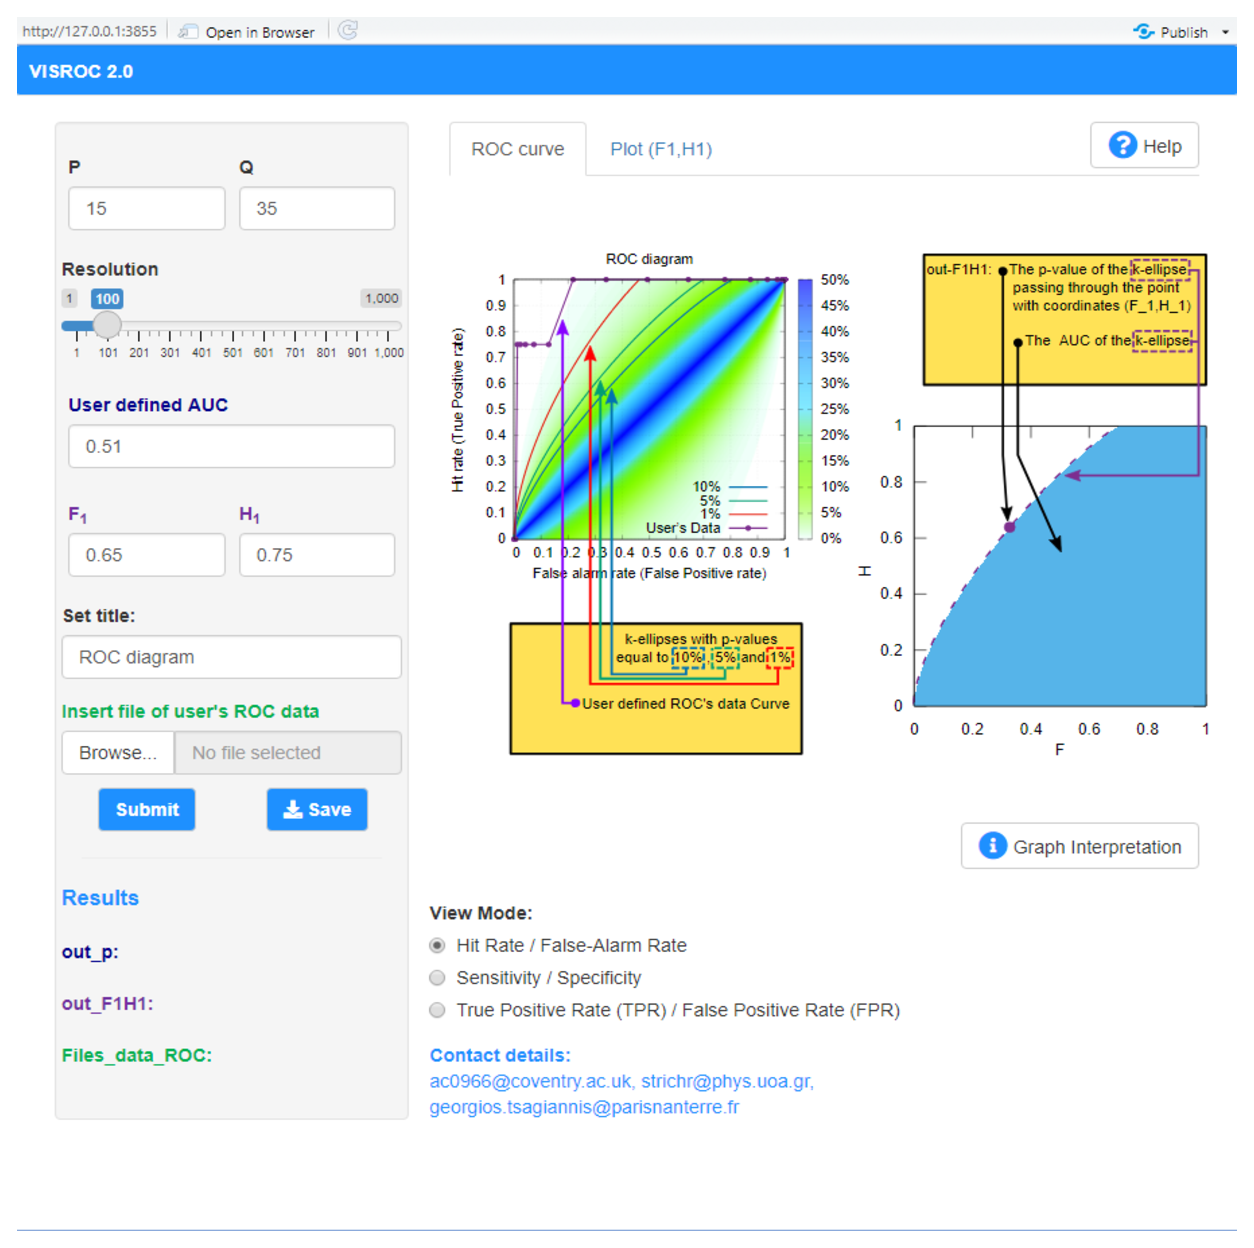
\includegraphics[scale=0.6]{Figure1.eps}
\caption{VISROC 2.0 GUI for the $R$ version of the software.}\label{fig:1}
\end{figure}

\begin{figure}
\includegraphics[scale=0.55]{Figure2.eps}
\caption{An example run using the $R$ version of VISROC 2.0. By clicking on the circled selection, the window changes to the picture on the top.}\label{fig:2}
\end{figure}

\begin{figure}
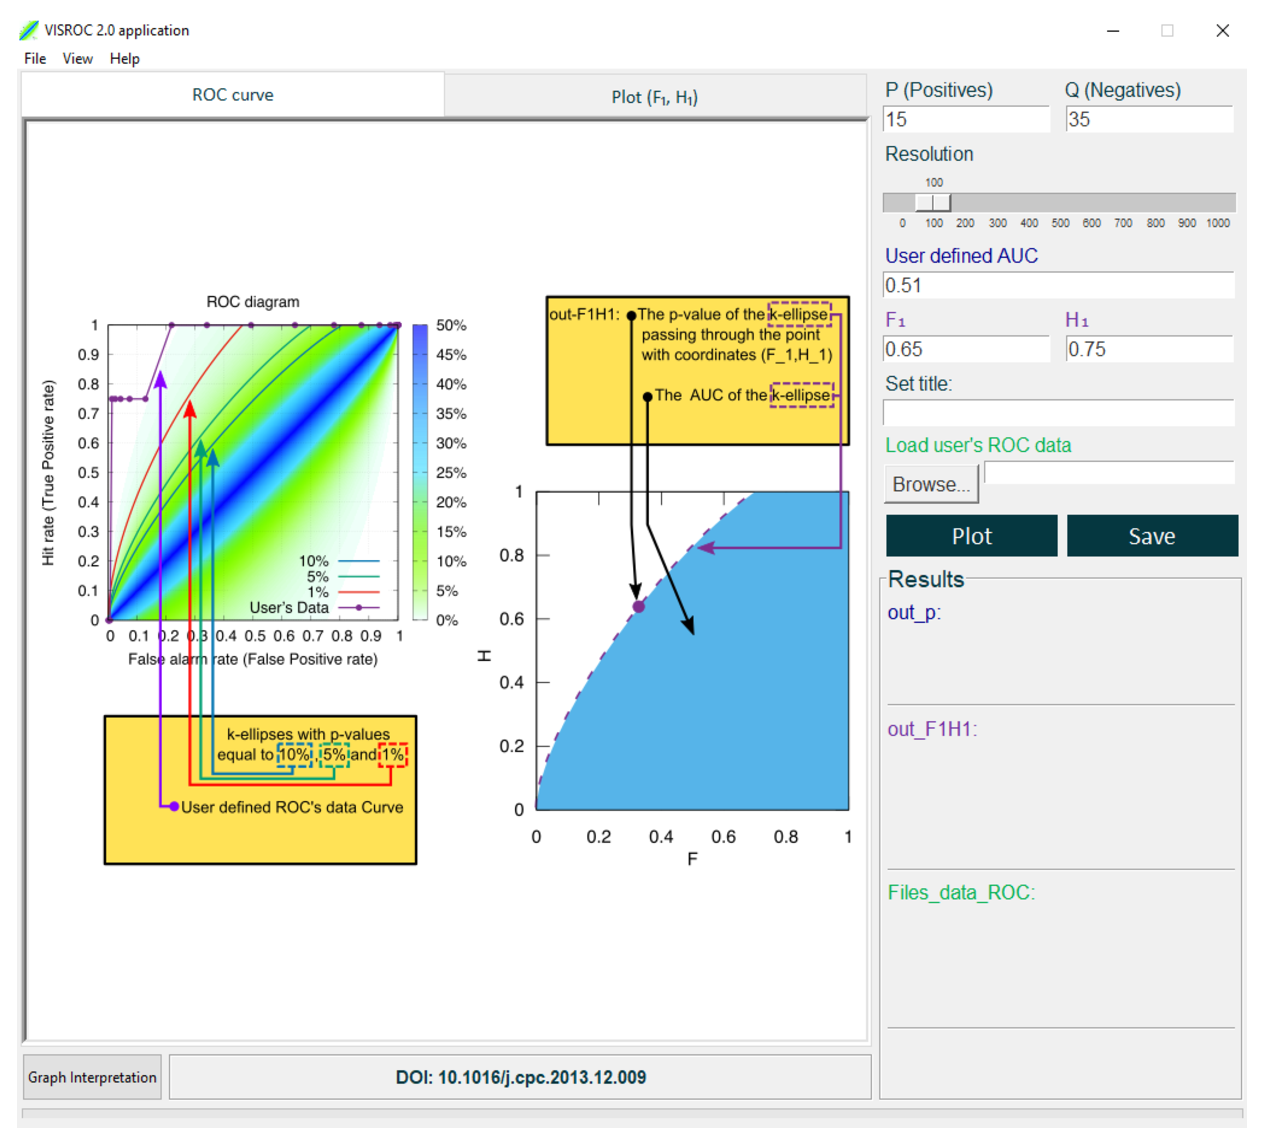
\includegraphics[scale=0.6]{Figure3.eps}
\caption{VISROC 2.0 GUI for the $Python$ version of the software.}\label{fig:3}
\end{figure}

\begin{figure}
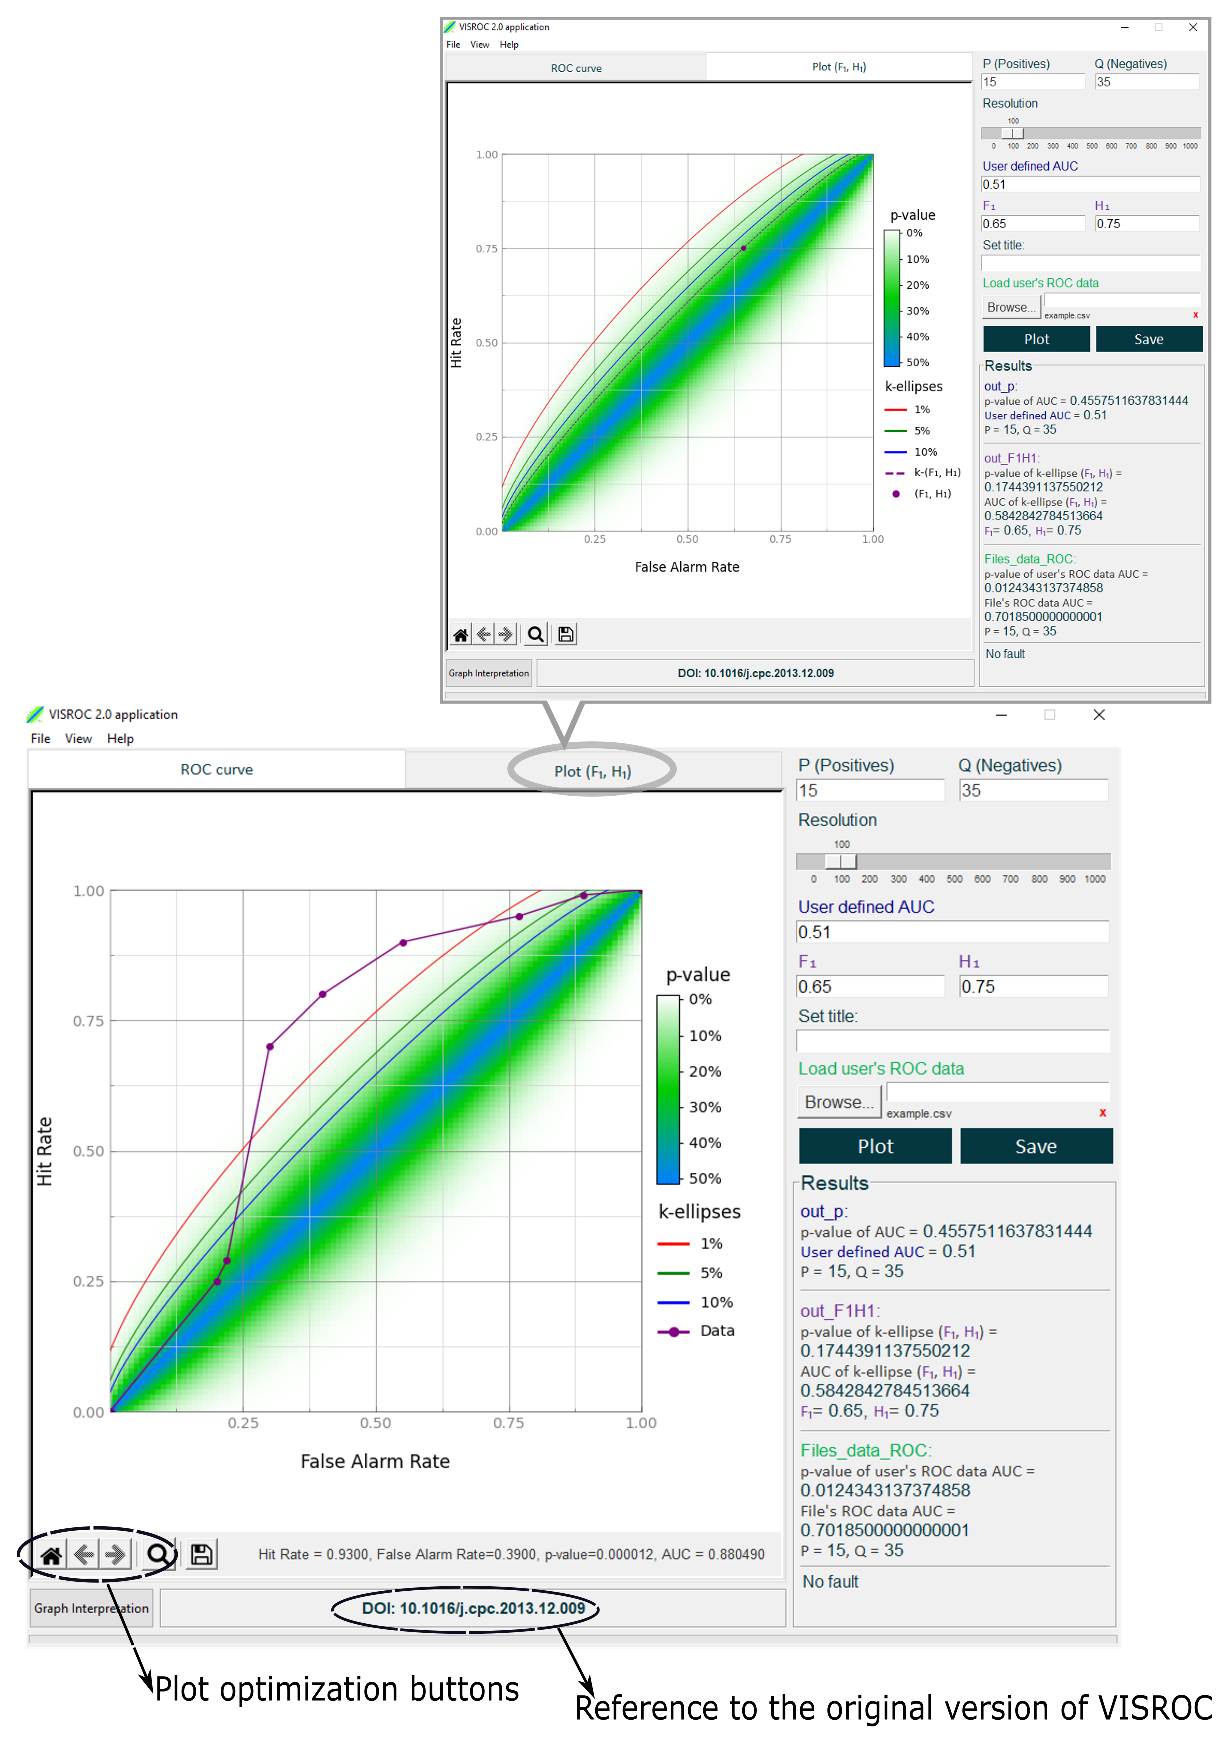
\includegraphics[scale=0.55]{Figure4.eps}
\caption{An example run using the $Python$ version of VISROC 2.0. By clicking on the circled selection, the window changes to the picture on the top.}\label{fig:4}
\end{figure}

\begin{figure}
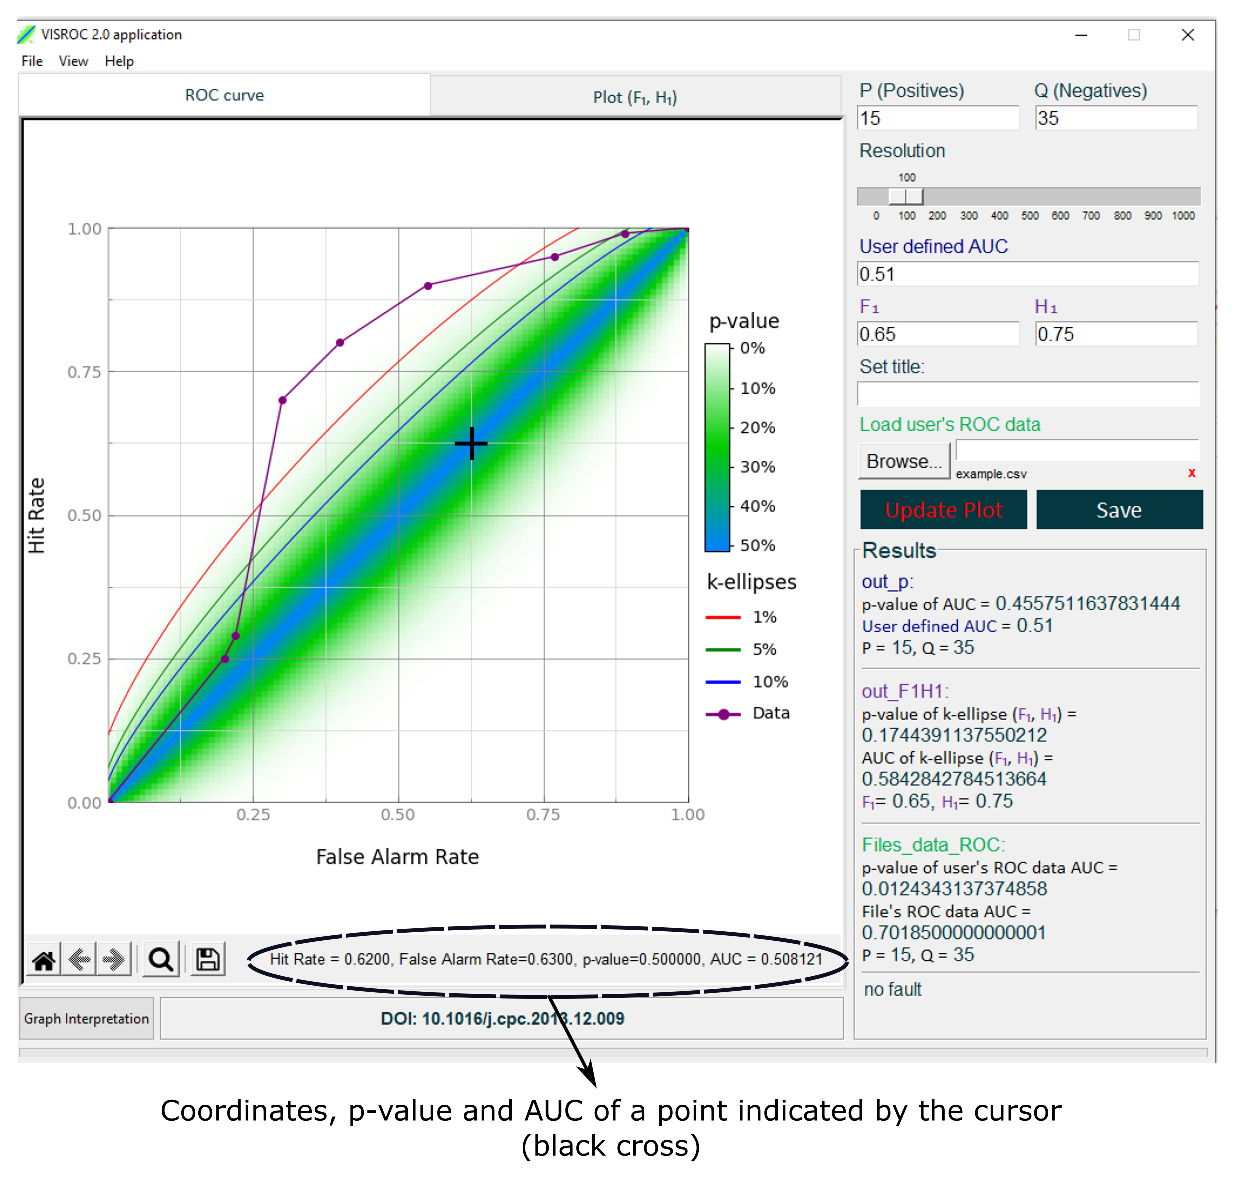
\includegraphics[scale=0.6]{Figure5.eps}
\caption{By passing the cursor over a specific point in the $Python$ version of VISROC 2.0, the user can see its coordinates, $p$-value and AUC.}\label{fig:5}
\end{figure}

\end{document}

%%
%% End of file 
